\begin{center}
\textsc{\Large Laboratorio 14}~\\
{\large Vídeo Juegos, Físicas, Programación}~\\
\emph{Física en Vídeo Juegos, Partículas y Proyectiles}
\end{center}

\section{Pre-Laboratorio}
\todo[inline]{Por hacer.}

\section{Introducción}
\setlength\intextsep{0pt}
\begin{wrapfigure}[8]{r}{0.4\linewidth}
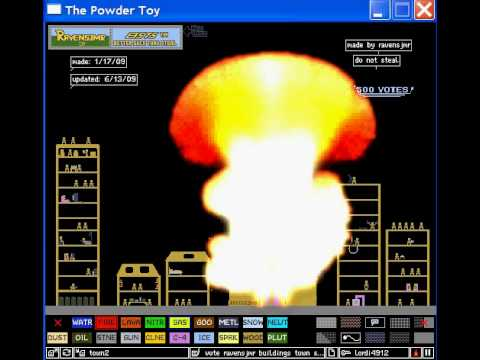
\includegraphics[width=\linewidth]{semana14/powdertoy.jpg}
\caption{\emph{Powder Toy} un juego 2D que utiliza sistemas de particulas.}
\label{fig:particles}
\end{wrapfigure}
Para agregar realismo, nuevas mecánicas o mayor calidad visual se introducen leyes físicas dentro del motor de juego, es mayormente usado en juegos tridimensionales. Estas nuevos efectos se introducen en forma de simulaciones las cuales son aproximaciones de fenómenos reales utilizando valores discretos \cite{ian_gamephysics}.

\section{Sistemas de Partículas}
Es una técnica utilizada en físicas de juegos y computación gráfica en la que se usa una cantidad grande de pequeños \emph{sprites} u otros objetos visuales para simular ciertos fenómenos como sistemas altamente caóticos, fenómenos naturales o procesos causados por reacciones químicas \cite{vanderburg_particlesystem}. 

Algunos ejemplos de fenómenos que son replicados utilizando sistemas de partículas, es el fuego, explosiones, humo, agua en movimiento (como cascadas de agua), nubes, estrellas, galaxias, etc. Es también común su uso para efectos visuales abstractos (ver \ref{fig:particles}).
\section{Proyectiles}
\setlength\intextsep{0pt}
\begin{wrapfigure}[10]{l}{0.4\linewidth}
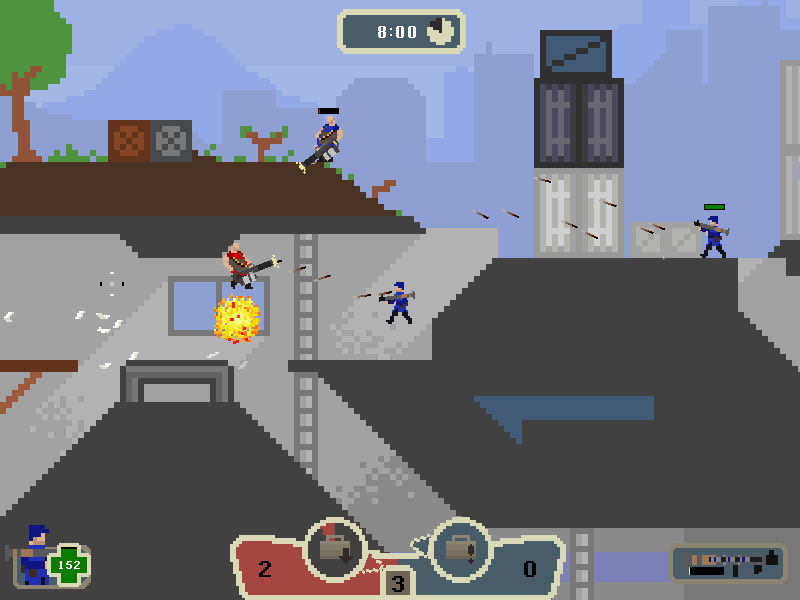
\includegraphics[width=\linewidth]{semana14/Gang_Garrison_2.png}
\caption{Gang Garrison 2 un shooter 2D basado en Team Fortress 2, distintas clases tienen distintos tipos de proyectiles.}
\label{fig:ganggarrison2}
\end{wrapfigure}

En algunos vídeo juegos los objetos de tipo proyectil son sometidos a simulaciones físicas o aproximaciones. Usualmente en la programación de un juego un proyectil sigue una linea recta o parabólica y en caso de colisión se inicia algún evento. Otros juegos consideran factores que afectan la trayectoria del proyectil tales como resistencia y/o dirección al viento, velocidad de proyectil (en vez de una trayectoria inmediata el proyectil posee una velocidad en espacio), gravedad, entre otros \cite{fifa_physics}.~\\

\section{Actividad}
\todo[inline]{Por hacer.}